%---------change this every homework
\def\yourid{yl4df}
\def\collabs{mw5ew}
\def\sources{list any sources, e.g.\ Cormen, et al, Introduction to Algorithms}
% NOTE: To specifically cite your sources, include your bibliography.bib file from
% homework 0 when LaTeXing your document (or upload it to Overleaf with this document)
% and then uncomment the penultimate last two lines of this file to display the
% bibliography.
% -----------------------------------------------------
\def\duedate{Sunday, April 12 at 11p}
\def\duelocation{via Collab}
\def\hnumber{7}
\def\course{{cs4102 - algorithms - spring 2020}}%------
%-------------------------------------
%-------------------------------------

\documentclass[10pt]{article}
\usepackage[colorlinks,urlcolor=blue]{hyperref}
\usepackage[osf]{mathpazo}
\usepackage{tikz}
\usetikzlibrary{arrows}
\usepackage{amsmath,amsfonts,graphicx}
\usepackage{latexsym}
\usepackage[top=1in,bottom=1.4in,left=1.25in,right=1.25in,centering,letterpaper]{geometry}
\usepackage{color}
\definecolor{mdb}{rgb}{0.1,0.6,0.4} 
\definecolor{cit}{rgb}{0.05,0.2,0.45} 
\pagestyle{myheadings}
\markboth{\yourid}{\yourid}
\usepackage{clrscode}
\usepackage{url}
\usepackage{tabularx,booktabs}
\newcolumntype{Y}{>{\centering\arraybackslash}X}

\newenvironment{proof}{\par\noindent{\it Proof.}\hspace*{1em}}{$\Box$\bigskip}
\newcommand{\handout}{
   \renewcommand{\thepage}{Homework \hnumber~-~\arabic{page}}
   \noindent
   \begin{center}
      \vbox{
    \hbox to \columnwidth {\sc{\course} \hfill}
    \vspace{-2mm}
       \hbox to \columnwidth {\sc due \MakeLowercase{\duedate} \duelocation\hfill {\Huge\color{mdb}H\hnumber(\yourid)}}
      }
   \end{center}
   \vspace*{1mm}
   \hrule
   \vspace*{1mm}
    {\footnotesize \textbf{Collaboration Policy:} You are encouraged to collaborate with up to 4 other students, but all work submitted must be your own {\em independently} written solution. List the computing ids of all of your collaborators in the comments at the top of the tex file. {\color{cit} You \textbf{are} permitted to collaborate through online tools such as Google Docs, interactive whiteboards, Google Meet, Google Hangouts, Zoom, Skype, etc, however you \textbf{must} limit written/typed details to high-level algorithm design.  Each person is responsible for taking those ideas and turning them into pesudocode and a writeup. Do \textbf{NOT} copy and paste from shared documents, which includes re-typing verbatim or trying to disguise text that you are essentially copying.  Over-collaboration of that form is fairly easy to detect with plagiarism tools.} {\color{red}\textbf{Do not seek published or online solutions, including pseudocode, for this assignment.}} If you use any published or online resources (which may not include solutions) when completing this assignment, be sure to cite them. Do not submit a solution that you are unable to explain orally to a member of the course staff. Any solutions that share similar text/code will be considered in breach of this policy. Please refer to the syllabus for a complete description of the collaboration policy.
   \vspace*{1mm}
    \hrule
    \vspace*{2mm}
    \noindent
    \textbf{Collaborators}: \collabs\\
    \textbf{Sources}: \sources}
    \vspace*{2mm}
    \hrule
    \vskip 2em
}
\newcommand{\solution}[1]{\medskip\noindent\textbf{Solution:}#1}
\newcommand{\bit}[1]{\{0,1\}^{ #1 }}
\newcommand{\answer}[1]{\color{blue}\hfill\break\\\noindent\textbf{#1}\color{black}\hfill\break}
\newcommand{\points}[1]{\normalfont{[#1 points]}}
%\dontprintsemicolon
%\linesnumbered
\newtheorem{problem}{\sc\color{cit}problem}
\newtheorem{extra}{\sc\color{cit}extra credit}
\newtheorem{practice}{\sc\color{cit}practice}
\newtheorem{lemma}{Lemma}
\newtheorem{definition}{Definition}
\newtheorem{theorem}{Theorem}

\newcommand{\Z}{\mathbb{Z}} % This might be useful for Integers!

\begin{document}
\thispagestyle{empty}
\handout

%----Begin your modifications here

\begin{problem}Unique Minimum Spanning Trees \points{14} \end{problem}

    \begin{enumerate} 
        \item Show that a graph $G=(V,E)$ has a unique minimum spanning tree $T$ if, for every cut of $G$, there is a unique minimum weight edge crossing the cut.  
        \begin{proof}
        Prove by contradiction. Suppose there exist two different MSTs, $T$ and $T'$. Let us sat that they differ by at least one edge $e$. That is, $e \in T$ and $e \notin T'$. If we remove $e$, $T$ will be disconnected, so there exists a cut $(S, V-S)$ which $e$ crosses. Since $e \in T$, we can say $e$ is a minimum weight edge. For $e \notin T'$, we can still find a path in $T'$ connecting the two vertices which are connected by $e$ in $T$, because $T'$ is MST. This implies there exists an edge $e' \in T'$ crossing the cut $(S, V-S)$ and $e'$ is a minimum weight edge since $T'$ is a MST. Since we know that for every cut of $G$ there is a unique minimum weight edge crossing the cut, we can say $e=e'$. This lead to contradiction regarding that $e \notin T'$. We can conclude that the graph has a unique minimum spanning tree.
        \end{proof}
        \item Show the converse is not true by providing a counterexample.
        \begin{proof}
        \\
        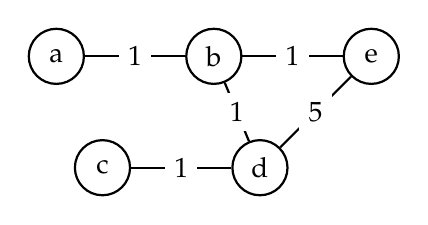
\begin{tikzpicture}[-,>=stealth',node distance=2cm,thick,node/.style={circle,draw,minimum size=7mm}]
 % 5 nodes
 \node[node] (a) {a};
 \node[node] (b) [right of=a] {b};
 \node[node] (c) [below left of=b] {c};
 \node[node] (d) [right of=c] {d};
 \node[node] (e) [above right of=d] {e};

 % edges between some nodes with weights
 \path[every node/.style={
 fill=white}]
 (a) edge [] node[] {$1$} (b)
 (b) edge [] node[] {$1$} (e)
     edge [] node[] {$1$} (d)
 (c) edge [] node[] {$1$} (d)
 (d) edge [] node[] {$5$} (e);
\end{tikzpicture}
\\
The graph has a unique MST with edge $\{(c,d),(d,b),(b,a),(b,e)\}$. However, for the cut $((a,b),(c,d,e))$, there are two minimum weight edges crossing the cut, namely $(b,d)$ and $(b,e)$. Thus, the converse is not true.
\end{proof}
    \end{enumerate}

\begin{problem}Divide and Conquer with MSTs \points{13} \end{problem}

Professors Horton and Hott have been discussing minimum spanning trees and attempting to create new algorithms to compute them.  Professor Horton claims to have created a divide and conquer algorithm as follows:  
\begin{quote}
    Given a graph $G = (V,E)$, partition the set of vertices $V$ into two sets $V_L$ and $V_R$ such that $|V_L|$ and $|V_R|$ differ by at most 1.  Let $E_L$ be the set of edges that are incident only on vertices in $V_L$ and $E_R$ be the set of edges incident only on vertices in $V_R$.  Recursively compute the minimum spanning tree on each of the two subgraphs $G_L = (V_L, E_L)$ and $G_R = (V_R, E_R)$, then select the minimum weight edge $e \in E$ that crosses the cut $(V_L, V_R)$.  Use $e$ to combine the two minimum spanning trees into a single minimum spanning tree for $G$.
\end{quote}
Help us to evaluate his algorithm.  Either prove that it correctly computes a minimum spanning tree of graph $G$ or provide a counterexample for which the algorithm fails.
        \begin{proof}
        The algorithm fails. Counterexample and explanation is provided as follows.\\
        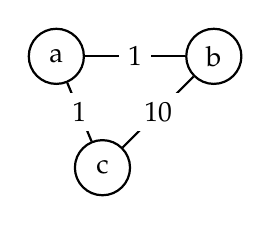
\begin{tikzpicture}[-,>=stealth',node distance=2cm,thick,node/.style={circle,draw,minimum size=7mm}]
 % 3 nodes
 \node[node] (a) {a};
 \node[node] (b) [right of=a] {b};
 \node[node] (c) [below left of=b] {c};

 % edges between some nodes with weights
 \path[every node/.style={
 fill=white}]
 (a) edge [] node[] {$1$} (b)
 (b) edge [] node[] {$10$} (c)
 (c) edge [] node[] {$1$} (a);
\end{tikzpicture}
\\
 Following the algorithm, we partition $V$ into $V_L=(a)$ and $V_R=(b,c)$. Then $E_L=()$ and $E_R=((b,c))$. For $G_L$, the MST is just the vertex $a$. For $G_R$, the MST only consists of the edge $(b,c)$. Then select the minimum weight edge $(a,b)$ to combine two MSTs, so the final MST consists of edges $(a,b)$ and $(b,c)$. We also could use $(a,c)$ to perform combining, but the final conclusion does not differ, so I use $(a,b)$ to illustrate. However, the result is incorrect because the MST for this graph has the edges $(a,b)$ and $(a,c)$. Thus, the algorithm fails.
\end{proof}

\begin{problem} Counting Shortest Paths \points{13} \end{problem}
Given a graph $G = (V, E)$, and a starting node $s$, let $\ell(s, t)$ be the length of the shortest path in terms of number of edges between $s$ and $t$. Design an algorithm that computes the number of distinct paths from $s$ to $t$ that have length exactly $\ell(s, t)$.\\
\\
The algorithm is modified from BFS. For each node, we created two arrays, lpath[] and npath[]. lpath[] stores the length of shortest path from $s$ to the current node. npath[] stores the number of shortest path from $s$ to the current node. For all nodes, initialize lpath$=\infty$ and npath$=0$. We begin the algorithm on $s$, so set lpath[$s$]$=0$ and npath[$s$]$=1$. Then we transverse like BFS. For every adjacent node $u$ of each vertex $v$ in $G$, we consider two cases. If lpath[$u$] $>$ lpath[$v$]$+ 1$, we update lpath[$u$] $=$ lpath[$v$]$+ 1$ and set npath[$u$]=napth[$v$]. If lpath[$u$] $=$ lpath[$v$]$+ 1$, then npath[$u$]=napth[$v$]$+$npath[$u$]. The algorithm returns npath[$t$]. The pseudo-code is provided. \\
$\mathtt{CSP}(G, s)$:\\
\-\hspace{0.5cm} Initialize a flag $d_v= 0$, lpath[$v$]$=\infty$ and npath[$v$]$=0$ for each node $v$\\
\-\hspace{0.5cm} Initialize the start node $s$ as lpath[$s$]$=0$ and npath[$s$]$=1$\\
\-\hspace{0.5cm} Q.push(s)\\
\-\hspace{0.5cm} While Q is not empty:\\
\-\hspace{1cm} v=Q.pop() and set $d_v=1$\\
\-\hspace{1cm} For each $u \in V$ such that $(u, v) \in E$:\\
\-\hspace{1.5cm} If $d_u=0$:\\
\-\hspace{2cm} Q.push(u)\\
\-\hspace{1.5cm} If lpath[$u$] $>$ lpath[$v$]$+ 1$:\\
\-\hspace{2cm} lpath[$u$] $=$ lpath[$v$]$+ 1$\\
\-\hspace{2cm} npath[$u$]=napth[$v$]\\
\-\hspace{1.5cm} Else if lpath[$u$] $=$ lpath[$v$]$+ 1$:\\
\-\hspace{2cm} npath[$u$]=napth[$v$]$+$npath[$u$]\\
\-\hspace{0.5cm} return npath[$t$]\\
\newpage
\begin{problem} Lecture Review Questions \points{20}\end{problem}

    \begin{enumerate}
        \item If you were given a list of nodes $P$ and you needed to determine if $P$ is a valid path in graph $G = (V,E)$, which of the two graph data structures for $G$ would be more efficient, or would they be the same? (Name one of the choices, or say "same". No explanation required.)
            \answer{Adjacent Matrix} % put your answer inside this command

        \item If a graph is not connected, can it have an MST? (Answer ``yes'' or ``no.'' No explanation needed.)
            \answer{No} % put your answer inside this command

        \item Briefly explain how Prim's algorithm insures that an edge that results in a cycle is never selected.
            \answer{It always selects the edge which connects a node in tree with a node not in tree } % put your answer inside this command

        \item Which of the following are true? If nodes in a graph are partitioned by a cut into two subsets, $S$ and $V-S$, then a set of edges that respects this cut can contain:
            \begin{itemize}
                \item[a) ] an edge $(a,b)$ where $a \in V$ and $b \in V-S$.
                \item[b) ] two edges $(a,b)$ and $(c,d)$ where $a$ and $b$ are in $V$ and $c$ and $d$ are in $V-S$
                \item[c) ] only edges where all the edges' nodes are either in $V$ or in $V-S$
            \end{itemize}
            \answer{b} % put your answer inside this command

        \item How is the key stored in the heap for Dijkstra's shortest path algorithm different that the key stored in Prim's MST algorithm?
            \answer{Instead of just the weight of an edge, Dijkstra's SP algorithm stores key as the total weight of shortest path from start node to the current node. } % put your answer inside this command

        \item If you had an unusual weighted graph where all the edge-weights had the same value, name an algorithm other than Dijkstra's shortest path algorithm that you could easily use to find the shortest path between two nodes. Would this algorithm's time-complexity be better or worse than using Dijkstra's algorithm for this purpose?
            \answer{We could use BFS. It is better regarding time-complexity. BFS takes $O(V+E)$ whereas Dijkstra takes $O((V+E)\log V)$} % put your answer inside this command

    \end{enumerate}


%%%%%%%%%%%%%%%%%%%%%%%%%%%%%%%%%%%%%%%%%%%%%%%%%%%%%%%%%%%%%%%%%%%%%%%%%%%%%%
% EXTRA CREDIT OPPORTUNITY
\newpage
\noindent
   \begin{center}
      \vbox{
          \hbox to \columnwidth {\hfill {\sc \Huge\color{mdb}EC2(\yourid)}}
      }
   \end{center}
   \vspace*{1mm}
   \hrule
   \vspace*{1mm}
    {\footnotesize \textbf{Extra Credit Instructions:} For each of the next three written homeworks (HW6, HW7, HW9), you will be given an extra credit problem, with the opportunity to replace one homework at the end of the course.  Combined, the extra credit portions are worth $60$ points---the same as one normal homework assignment.  Each Extra Credit portion (EC1, EC2, EC3) will be combined into one \emph{optional} replacement homework, meaning that the total scored out of all $60$ extra credit points will replace your lowest homework grade for the semester.  Note: this extra credit will \textbf{not} be applied to this homework (HW\hnumber).  To make the most of this opportunity, you should commit to solving \textbf{all} extra credit portions for the next three homework assignments.}
   \vspace*{1mm}
    \hrule
    \vspace*{2mm}
    \noindent
    {\footnotesize Since the extra credit is optional, no office hours will be provided to aid in solving the additional \emph{optional} problems.}
    \vspace*{2mm}
    \hrule
    \vskip 2em

\begin{extra} Martian Morels \end{extra}

\MakeUppercase{NEWSFLASH: subterranean humanoid race discovered on Mars!} 

\noindent Since the Martians live in caves, their diet consists of a variety of Martian mushrooms. The tastiest is the Martian Morel, said to be more delicious than any food on Earth. Problematically, one subspecies of the Martian Morel is deathly toxic to humans. The Martians seem capable of distinguishing between toxic and edible mushrooms, but we humans need to verify that they can do so consistently before we can market the mushrooms to humans. More problematically, the Martian language is unlike any human languages, so the only of their words we have learned so far are ``same'', ``different'', and ``uncertain''.

We have $n$ samples of Martian morels $s_1, ..., s_n$ each of which are either edible or toxic (we don't know which for any). A Martian was given all $n^2$ possible pairs of samples $(s_i, s_j)$. The Martian then decided whether each sample's mushrooms were (a) the same (both edible or both toxic), (b) different (one edible and one toxic), or (c) that the Martian was uncertain. (All pairs were tested, but not all have ``same'' or ``different'' decisions).

At the end of the testing, the Martian decided that a total of $m$ pairs were ``same'' or ``different''. Give an algorithm that determines whether these $m$ are consistent. The decisions are consistent if there is a way to label each sample $s_i$ with ``edible'' or ``toxic'' such that if the Martian indicated the pair $(s_i, s_j)$ was ``same'' our labels for $s_i,s_j$ matched, and if the Martian indicated the pair $(s_i, s_j)$ was ``different'' our labels for $s_i,s_j$ differed. Your algorithm should run in time $O(m+n)$.
\\
Algorithm:
\begin{enumerate}
    \item Construct a graph using $n$ samples as nodes and $m$ judgements as edges. If the judgement is "same", then we set the weight of that edge is 1. If the judgement is "different", then we set the weight of that edge is -1. If there are multiple edges between two nodes, we return false if different values appear among them. Pick up a start node $s$. It does not matter whether you set it to "edible" or "toxic", so I just set it to "edible". Mark it as visited. Then we transverse the graph using BFS. If the graph is no connected, we apply the algorithm on each connected part of it. 
    \item If a node is NOT visited, we assign "edible" or "toxic" based on the judgement. That is, for neighbor node $x$ of node $n$, if edge weight is 1, we assign the same label to $x$ as $n$. If edge weight is -1, we assign the different label to $x$ from $n$. After assigning, we mark it visited.
    \item If a node is visited, we perform checking based on the judgement. That is, for neighbor node $x$ of node $n$, if edge weight is 1, we check whether $x$ and $n$ have same label. If not, return false. If edge weight is -1, we check whether $x$ and $n$ have different labels. If not, return false.
    \item After we run the algorithm to assign label for each node and check against each judgement, it returns true.
\end{enumerate}
Since we perform assigned on each node, it takes $O(n)$. Since we check against each judgement, it takes $O(m)$. Thus, the total running time is $O(n+m)$.\\
% Bibliography - uncomment the next two lines to cite your sources!
%\bibliographystyle{plain}
%\bibliography{bibliography}
\end{document}

